\documentclass[a4paper]{article}

%------------------------------------------------------------
\usepackage[a4paper, total={6in, 9in}]{geometry}
\usepackage{amsmath, amssymb}
\usepackage{booktabs}
\usepackage{caption}
\usepackage{enumitem}
\usepackage{graphicx}
\usepackage{float}
\usepackage{inconsolata}
\usepackage{listings}
\usepackage{mathtools}
\usepackage{pstricks-add}
\usepackage{siunitx}
\usepackage[most]{tcolorbox}
\usepackage{tikz, pgfplots}
\usepackage{epstopdf} %converting to PDF
\usepackage{hyperref}
\usepackage{xfrac}

\usetikzlibrary{shapes.geometric}
\usetikzlibrary{arrows}

%------------------------------------------------------------
\graphicspath{{./fig/}}
\pgfplotsset{compat=1.13}
%------------------------------------------------------------
\setlength{\parindent}{0in}

\lstdefinestyle{C++}{
	language=C++,
	basicstyle=\ttfamily,
	keywordstyle=\color{blue}\ttfamily,
	stringstyle=\color{red}\ttfamily,
	commentstyle=\color{green}\ttfamily,
	morecomment=[l][\color{magenta}]{\#},
	showstringspaces=false
}

%------------------------------------------------------------
\newtcblisting[auto counter]{sexylisting}[2][]{sharp corners, 
    fonttitle=\bfseries, colframe=gray, listing only, 
    listing options={basicstyle=\ttfamily,language=C++}, 
    title=Listing \thetcbcounter: #2, #1}

%------------------------------------------------------------
\lstset{language=C++,
        basicstyle=\ttfamily,
        keywordstyle=\color{blue}\ttfamily,
        stringstyle=\color{red}\ttfamily,
        commentstyle=\color{green}\ttfamily,
        morecomment=[l][\color{magenta}]{\#},
        showstringspaces=false
}
%------------------------------------------------------------
\tikzstyle{block} = [draw, fill=blue!20, rectangle, 
    minimum height=3em, minimum width=3em]
\tikzstyle{sum} = [draw, fill=blue!20, circle, node distance=1cm]
\tikzstyle{input} = [coordinate]
\tikzstyle{output} = [coordinate]
\tikzstyle{pinstyle} = [pin edge={to-,thin,black}]

%------------------------------------------------------------
\newlength{\arrow}
\settowidth{\arrow}{\scriptsize$1000$}

\newcommand*{\myrightarrow}[1]{\xrightarrow{\mathmakebox[\arrow]{#1}}}

\newcommand{\uvec}[1]{\boldsymbol{\hat{\textbf{#1}}}}

%------------------------------------------------------------

\begin{document}
\title{ENG252 Dynamics: Practical 2}
\author{Shane Reynolds}
\maketitle

\section{Introduction}
Dynamics of physical systems can be analysed by considering forces acting on the system. Whilst this method typically yields solutions in theory, it can be cumbersome to put into practice. An alternative approach, whereby system energies are considered, is often faster and conceptually easier to deal with. The simplest definition for energy is the ability to do work, where work, $W$, is defined as the application of force over a distance. More concretely, Giancolli defines this as the product of the magnitude of the displacement, $d$, multiplied by the component of a constant force parallel to the displacement, $F_{||}$. This is shown mathematically in equation (1).
\begin{equation}
W = F_{||}d
\end{equation}

The above definition has limited application since the object path may be non-linear, and the force variable, but we can use this to form a more sophisticated understanding. Suppose that a variable force $\boldsymbol{F}$ is applied to move an object along some path from $a$ to $b$, as shown in Figure 1. We note that as the force magnitude and direction changes, so too does the angle it makes with the path tangent. Two instances of the force are shown as $\boldsymbol{F_1}$ and $\boldsymbol{F_2}$, and the angles they make with the path tangent, $\theta_1$ and $\theta_2$, respectively.
\begin{figure}[h]
	\centering
	\begin{tikzpicture}
		\draw (0,0) .. controls (2,2) and (2,-2) .. (4,0);
		\draw[->, thick, magenta] (0,0) -- (0.5,1);
		\draw[->, thick, magenta] (2,0) -- (3,0.25);
		\fill (0,0) circle[radius=2pt] node[above left] {$a$};
		\fill (4,0) circle[radius=2pt] node[above right] {$b$};
		\node at (0.1,1) {$\boldsymbol{F_1}$};
		\node at (2.7,0.5) {$\boldsymbol{F_2}$};
	\end{tikzpicture}
	\caption{A variable force is applied to an object as it moves along a non-linear path from point a to b.}
\end{figure}

If we consider a small section of the path from $a$ to $b$, denoted as $\delta l_i$, we may assume the path is roughy linear and the force, $\boldsymbol{F_i}$, is constant in magnitude. Simple trigonometry can be applied to find the force component parallel to the linear section of the path, allowing us to approximate the change in work over $\delta l_i$ using equation (1).
\begin{equation}
\delta W_i = |\boldsymbol{F_i}| \cos\theta_i \delta l_i
\end{equation}

Considering all of the short linear sections along the path from $a$ to $b$ allows the summation of $\delta W_i$, expressed in equation (2), for each short section yielding an approximate of the work done for the entire path:
\begin{equation}
W = \sum_{i} \delta W_i = \sum_{i} |\boldsymbol{F_i}| \cos\theta_i \delta l_i
\end{equation}

In the limit, as $\delta l$ becomes infinitesimally small, equation (3) can be expressed as an integral:
\begin{equation}
W = \int_{a}^{b} |\boldsymbol{F}| \cos\theta dl
\end{equation}

Letting $d\boldsymbol{l}$ represent the infinitesimal displacement vector, equation (4) can be re-expressed using dot product notation:
\begin{equation}
W = \int_{a}^{b} \boldsymbol{F} \cdot d\boldsymbol{l}
\end{equation}

Decomposing force $\boldsymbol{F}$ using a rectilinear coordinate frame allows us to express the forces as:
\begin{equation}
\boldsymbol{F} = F_x \uvec{\i} + F_y \uvec{\j} + F_z \uvec{k}
\end{equation}

Similarly, we can re-express $d\boldsymbol{l}$ as:
\begin{equation}
d\boldsymbol{l} = dx \uvec{\i} + dy \uvec{\j} + dz \uvec{k}
\end{equation}

Hence, we can write (5) as:
\begin{equation}
W = \int_{a}^{b} F_x dx + \int_{a}^{b} F_y dy + \int_{a}^{b} F_z dz
\end{equation}

\subsection{Potential Energy}
\subsubsection{Gravitational Potential Energy}
Suppose that a mass $m$ is moved from some height $y_2$ to another height $y_1$, without acceleration, such that $y_2 > y_1$. If we only consider the force due to gravity, $F_g = mg$, acting on the mass then equation (8) allows the derivation of an expression for this work:
\begin{equation}
W_g = \int_{y_1}^{y_2} (mg) \ dy = mg(y_2 - y_1)
\end{equation}

The work is positive since the direction of movement is in the same direction as the force. Giancolli defines this as work due to gravitational potential energy, and goes on to define gravitational potential energy $V_g$, for some height $h$ above a reference point, as:
\begin{equation}
V_g = mgh
\end{equation}

\subsubsection{Elastic Potential Energy}
Suppose that a spring is stretched or compressed a distance $x$ from it's unstretched position. According to Giancolli, the spring exerts a force $F_s$ proportional to the stiffness coefficient, $k$, opposite to the direction of displacement:
\begin{equation}
F_s = -kx
\end{equation}

Letting the spring return to it's original unstretched state allows a spring force to act on an object attached to the spring, in the same direction of movement of the object. An equation for the work done by the spring can be expressed using (8) and (11).
\begin{equation}
W_e = \int_{0}^{x} kx \ dx = \frac{1}{2}kx^2
\end{equation}

Giancolli defines this as work due to elastic potential energy, and goes on to define elastic potential energy $V_e$, for some spring with linear displacement $x$, and stiffness coefficient $k$, as:
\begin{equation}
V_e = \frac{1}{2}kx^2
\end{equation}

\subsection{Conservation of Energy}

\subsection{Scope}

\section{Results}
A short section of elastic cord was used to capture experimental data on the cord's material properties. Two loops were tied in each end of the cord, so that one end could be attached to a retort stand, and the other end provided a location to place mass. The cord length was measured from knot to knot and was recorded as $0.47\si{\meter}$. Trials were undertaken placing successively larger masses on the cord. For each mass the cord was allowed to reach steady state elastic deformation, at which point the length was measured. The whole experiment was undertaken twice: lengths from the first experiment are labelled $\tilde{x}_1$; and lengths from the second experiment are labelled $\tilde{x}_2$. Experimental set up can be seen in Figure 2, and the tabulated results can be seen in Table 1.

\begin{figure}[h]
	\begin{minipage}{0.45\textwidth}
		\centering
		\frame{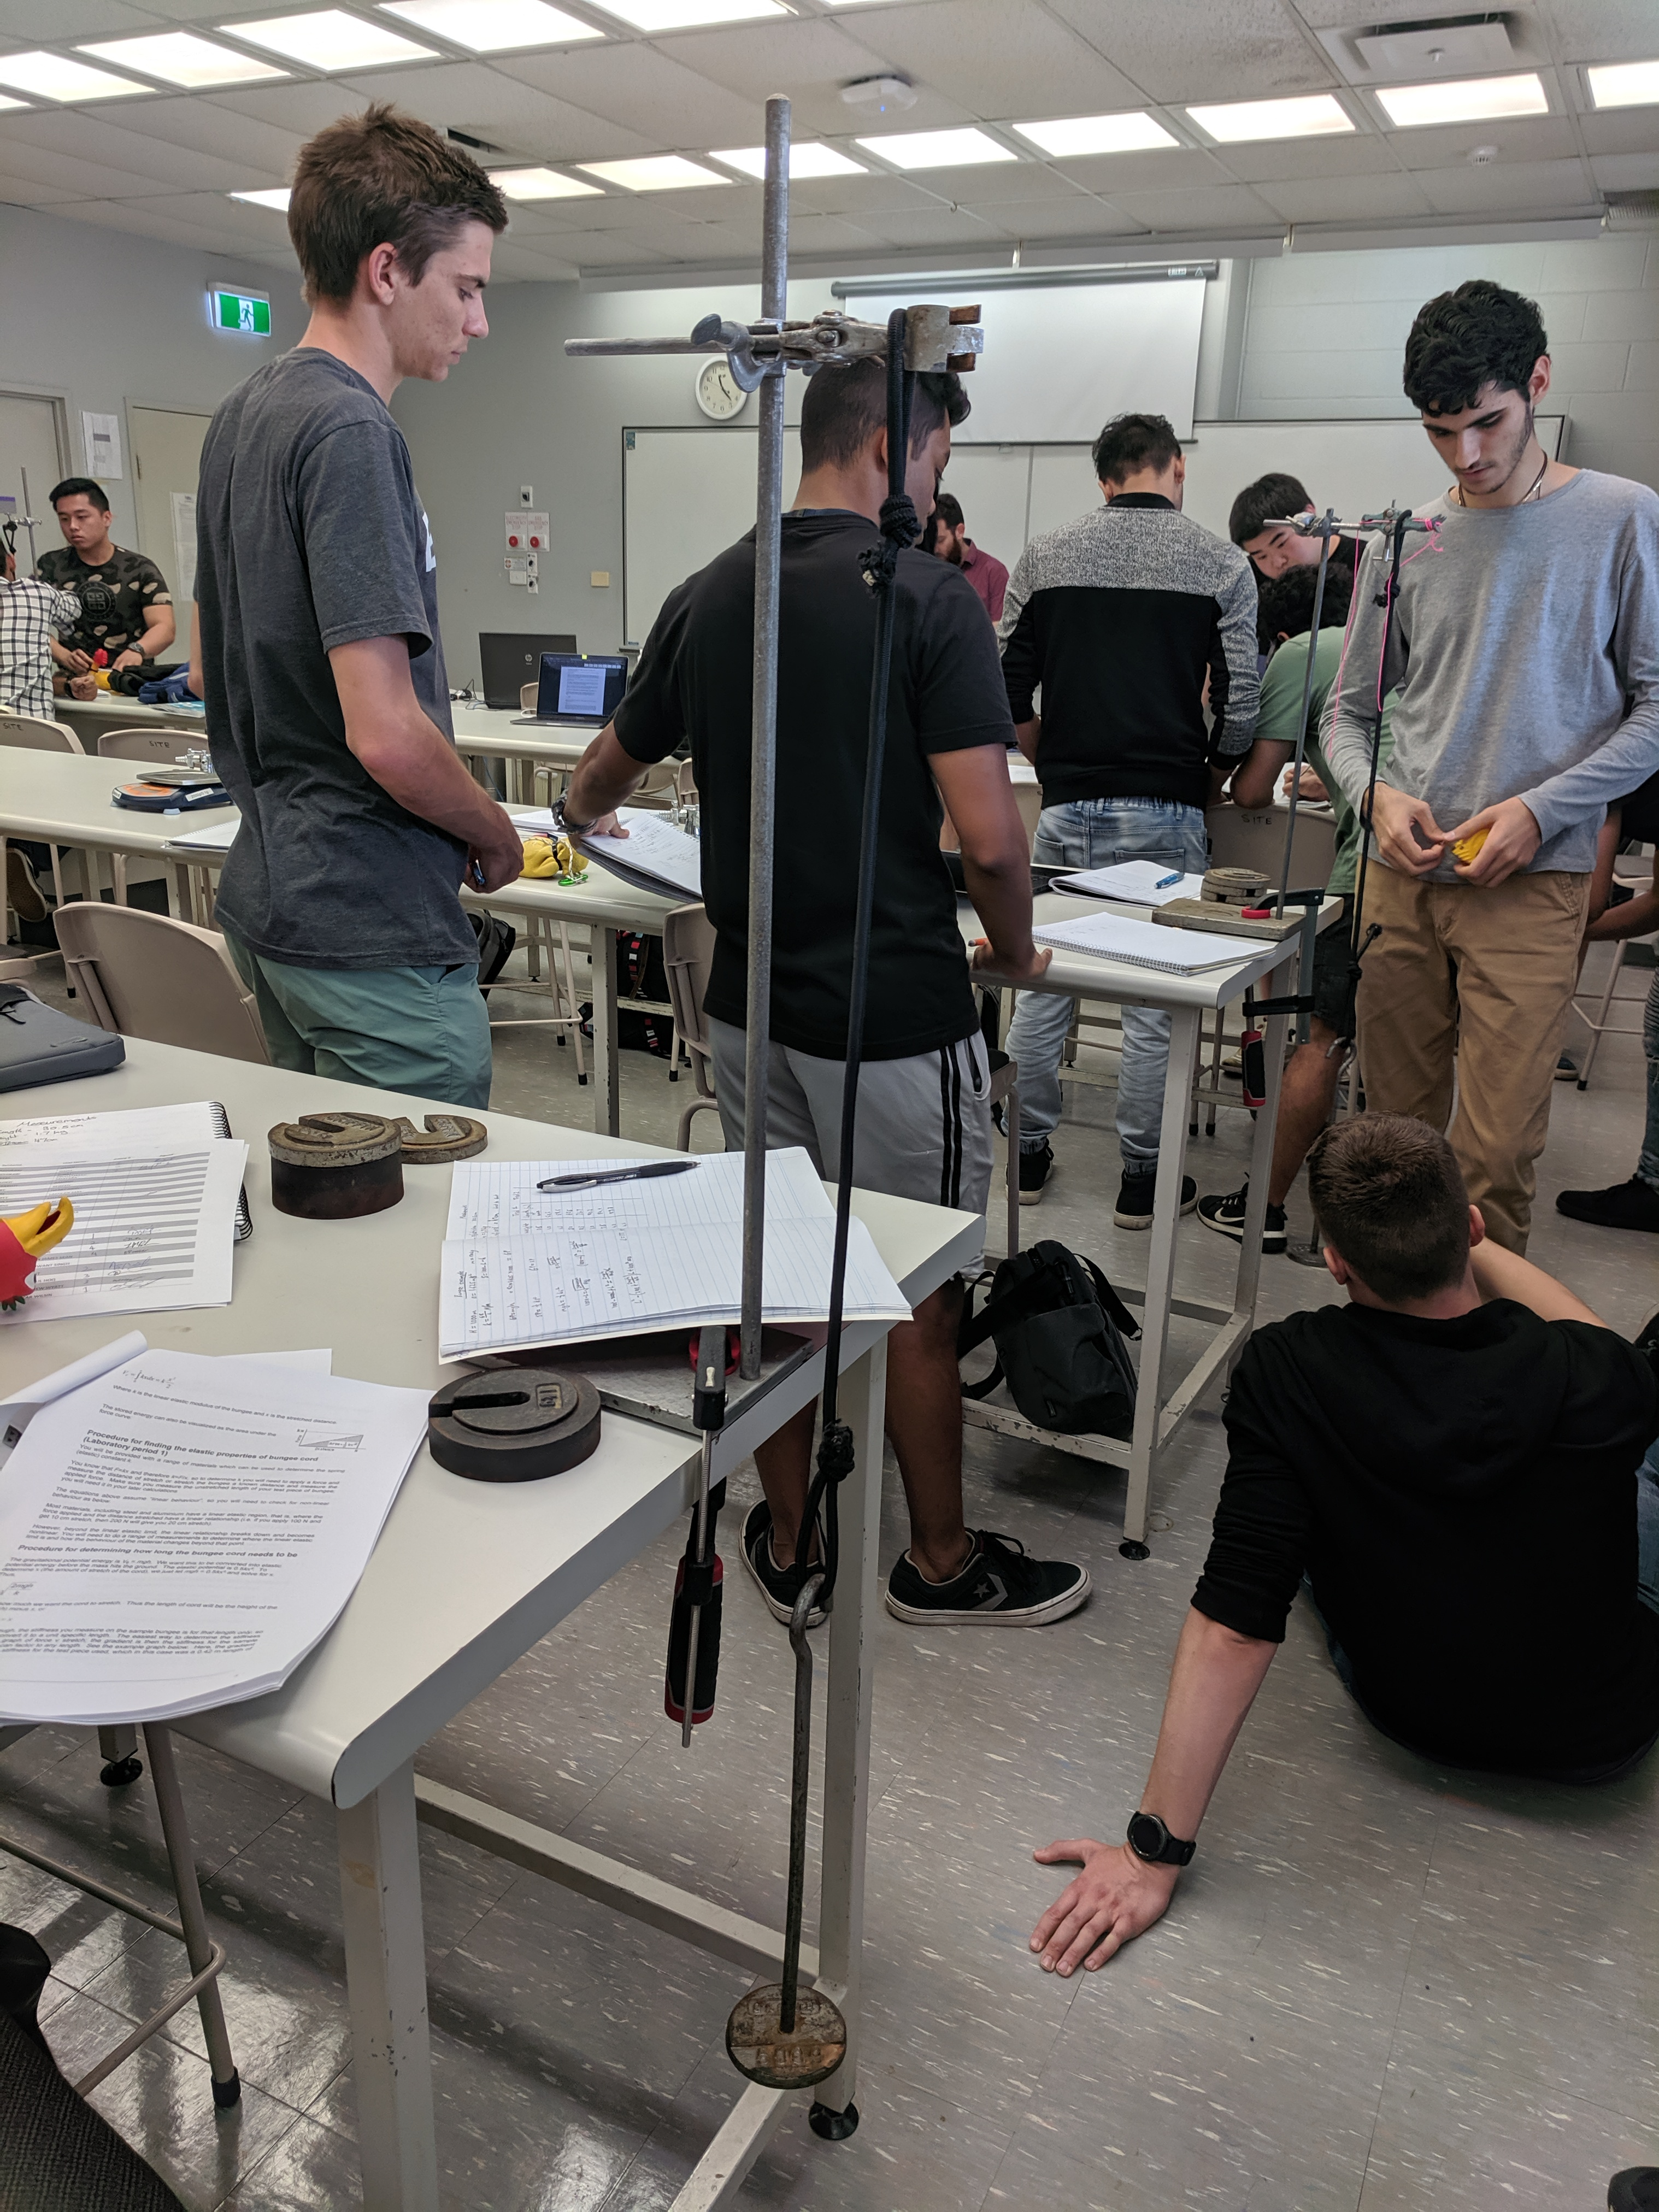
\includegraphics[scale=0.05]{result_1}}
		\caption{A terrible photo of the experimental set up highlighting cramped laboratory conditions often experienced with mass education}
	\end{minipage}
	\hspace{1cm}
	\begin{minipage}{0.45\textwidth}
			\centering
			\captionof{table}{Experimental data on elastic cord material properties were captured by placing successively larger masses on a known length of the cord and measuring the length of the cord at steady state elastic deformation}
			\begin{tabular}{rrr}
				\toprule
				Mass & Length 1 & Length 2\\
				$m$ $[\si{\kilogram}]$ & $\tilde{x}_1$ $[\si{\meter}]$ & $\tilde{x}_2$ $[\si{\meter}]$ \\
				\midrule
				0.00 & 0.47 & 0.47\\
				0.50 & 0.47 & 0.49\\
				1.00 & 0.51 & 0.53\\
				1.50 & 0.60 & 0.63\\
				2.00 & 0.69 & 0.72\\
				2.50 & 0.76 & 0.79\\
				3.00 & 0.80 & 0.83\\
				3.50 & 0.84 & 0.86\\
				4.00 & 0.87 & 0.88\\
				\bottomrule
			\end{tabular}
	\end{minipage}
\end{figure}


\section{Calculations}
Calculations are separated into two main subsections: determining the stiffness coefficient of the elastic cord used for the bungee jumping chicken; and the calculation of elastic cord length specified such that the bungee jumping chicken traverses the full balcony height without colliding with the ground.

\subsection{Determining Stiffness Coefficient, $k$}
The spring equation, derived from Hooke's law, states that under elastic deformation a force exerted by a spring, $F_s$, is opposite in direction and proportional to the springs displacement from it's unstretched state, $x$. The proportionality constant, referred to as the stiffness coefficient of the spring, is denoted by $k$. Mathematically the spring equation is expressed in equation (6).
\begin{equation}
F_s = -kx
\end{equation} 

A scatter plot of $(x, F_s)$ pairs can be used to approximate $k$ by fitting a linear model to the data using least squares. Equation (6) highlights that the linear regression model will need to be forced through the origin. To calculate $F_s$ we first note that at steady state elastic deformation the mass attached to the elastic cord is at rest. A free body diagram can be seen in Figure 3, where two forces are shown acting on the mass. Acting downwards is the force due to gravity, $F_g$; and acting upwards is an opposing force from the elastic cord, $F_s$. Since the mass is in static equilibrium we can calculate the magnitude of $F_s$ as follows:
\begin{align}
+ \uparrow \sum F &= 0 \nonumber \\
F_s - F_g &= 0 \nonumber \\
\therefore F_s &= F_g
\end{align} 

Given there will be no large excursions from the surface of Earth, it is reasonable to assume that force due to gravity is constant, and gravitational acceleration is equal to $9.81\si{\meter\per\second^2}$, which we denote by $g$. Given the mass attached to the cord is known, $F_s$ can be calculated using equation (7) and $F_g = mg$. Force calculations for all mass loadings are shown in Table 2.

\begin{figure}[h]
	\begin{minipage}{0.40\textwidth}
		\centering
		\begin{tikzpicture}
			\draw (0,0) circle (1cm);
			\draw[->, thick, magenta] (0,0) -- (0,-2);
			\draw[->, thick, magenta] (0,1) -- (0,3);
		\end{tikzpicture}
		\caption{A free body diagram of the mass in static equilibrium once the elastic cord has reached steady state elastic deformation.}
	\end{minipage}
	\hspace{0.5cm}
	\begin{minipage}{0.53\textwidth}
		\centering
		\captionof{table}{Calculated results for the force $F_s$ from the elastic cord, and the linear displacement from the cord's unstretched position, $x$.}
		\begin{tabular}{rrrrr}
			\toprule
			Mass & Force & Disp.  1 & Disp.  2 & Avg. Disp. \\
			$m$ $[\si{\kilogram}]$ & $F_s$ $[\si{\newton}]$ & $x_1$ $[\si{\meter}]$ & $x_2$ $[\si{\meter}]$ & $x$ $[\si{\meter}]$ \\
			\midrule
			0.00 &  0.00 & 0.00 & 0.00 & 0.00\\
			0.50 &  4.91 & 0.00 & 0.02 & 0.01\\
			1.00 &  9.81 & 0.04 & 0.06 & 0.05\\
			1.50 & 14.72 & 0.13 & 0.16 & 0.14\\
			2.00 & 19.62 & 0.22 & 0.25 & 0.23\\
			2.50 & 24.52 & 0.29 & 0.32 & 0.30\\
			3.00 & 29.43 & 0.33 & 0.36 & 0.35\\
			3.50 & 34.34 & 0.37 & 0.39 & 0.38\\
			4.00 & 39.24 & 0.40 & 0.41 & 0.41\\
			\bottomrule
		\end{tabular}
	\end{minipage}
\end{figure}

To calculate linear displacement, $x$, the unstretched cord length, $l_{act}$, is subtracted from the fully stretched cord length under loading, $\tilde{x}_i$. Mathematically, this calculation is expressed as follows:
\begin{equation}
x_i = \tilde{x}_i - l_{act}
\end{equation}

Linear displacement values calculated for each mass loading, using $l_{act} = 0.47\si{\meter}$ and equation (8), are shown in Table 2. Recall that experimental data was captured twice in order to reduce stochastic measurement error and hence there are two calculated columns, $x_1$ and $x_2$. The final column in the table is an average of the the $x_1$ and $x_2$ columns and represents the final linear displacement used in the scatter plot showin in Figure 4. 

\begin{figure}[h]
	\centering
	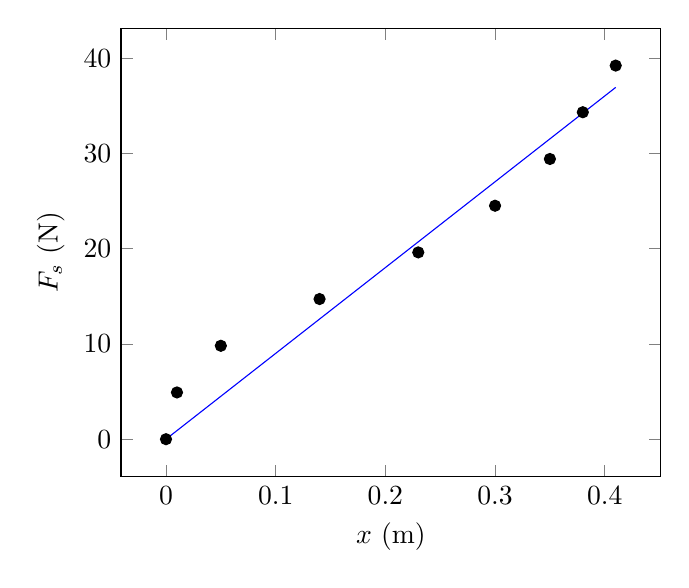
\begin{tikzpicture}
	\begin{axis}[xlabel=$x \ (\si{\meter})$,
				 ylabel=$F_s \ (\si{\newton})$]
	
	\addplot[only marks] coordinates {
		(0.00, 0.00)
		(0.01, 4.91)
		(0.05, 9.81)
		(0.14, 14.72)
		(0.23, 19.62)
		(0.30, 24.52)
		(0.35, 29.43)
		(0.38, 34.34)
		(0.41, 39.24)
	};
	
	\addplot[no marks, blue, domain=0:0.41] {90.12*x};
	
	\end{axis}
	\end{tikzpicture}
	\caption{Scatter plot showing the linear displacement from unstretched position on the horizontal axis and the resulting elastic force on the vertical axis. The blue line represents a linear model fit to the data, based on equation (14).}
\end{figure}

Least squares was used to fit a linear model to the scatter plot. Note that the model was forced through the origin. Graphically the model is depicted by the blue line in Figure 4. The reported regression equation can be seen in equation (9).
\begin{equation}
F_s = 90.12x \ \si{\newton}
\end{equation}

We note a stiffness coefficient of $90.12\si{\newton\per\meter}$ for the $0.47\si{\meter}$ length of bungee cord. The elastic cord material used for the bungee jumping chicken will be identical to that tested in the lab, however, the specified length will not be $0.47\si{\meter}$ so $k$ will need to be rescaled.

\subsection{Predicted Bungee Cord Length}
A rubber chicken of mass $m$, shown in Figure 5, will be tied to a section of elastic cord of length $L$. The other end of the cord will be fastened to a third story balcony. The chicken will be released, from rest, at a height $h$ above the ground. The chicken will fall the length $L$, at which point the elastic cord will begin to stretch by some amount $x$, arresting the fall and momentarily bringing the chicken to rest just above the ground. Additionally there are three other lengths that need to be considered prior to analysing the system: the chicken length, denoted as $l_1$; the length of a small tether at the base elastic cord to attached the chicken, denoted as $l_2$; and a small length of rope which clips the elastic cord to the balcony, denoted as $l_3$.\\

To determine the length $L$ such that the chicken will not collide with the ground we not that the sum of $L$, $l_1$, $l_2$, $l_3$, and $x$ must equal $h$. Mathematically this is described by equation (XXXX), and is shown graphically in Figure XXXX.
\begin{equation}
h = L + x + l_1 + l_2 + l_3
\end{equation}

More compactly, we can express equation (XXXX) as:
\begin{equation}
x = h - \bigg(L + \sum_{i=1}^{3} l_i \bigg)
\end{equation}

\begin{figure}[h]
	\centering
	\begin{minipage}[t]{0.45\textwidth}
		\centering
		\frame{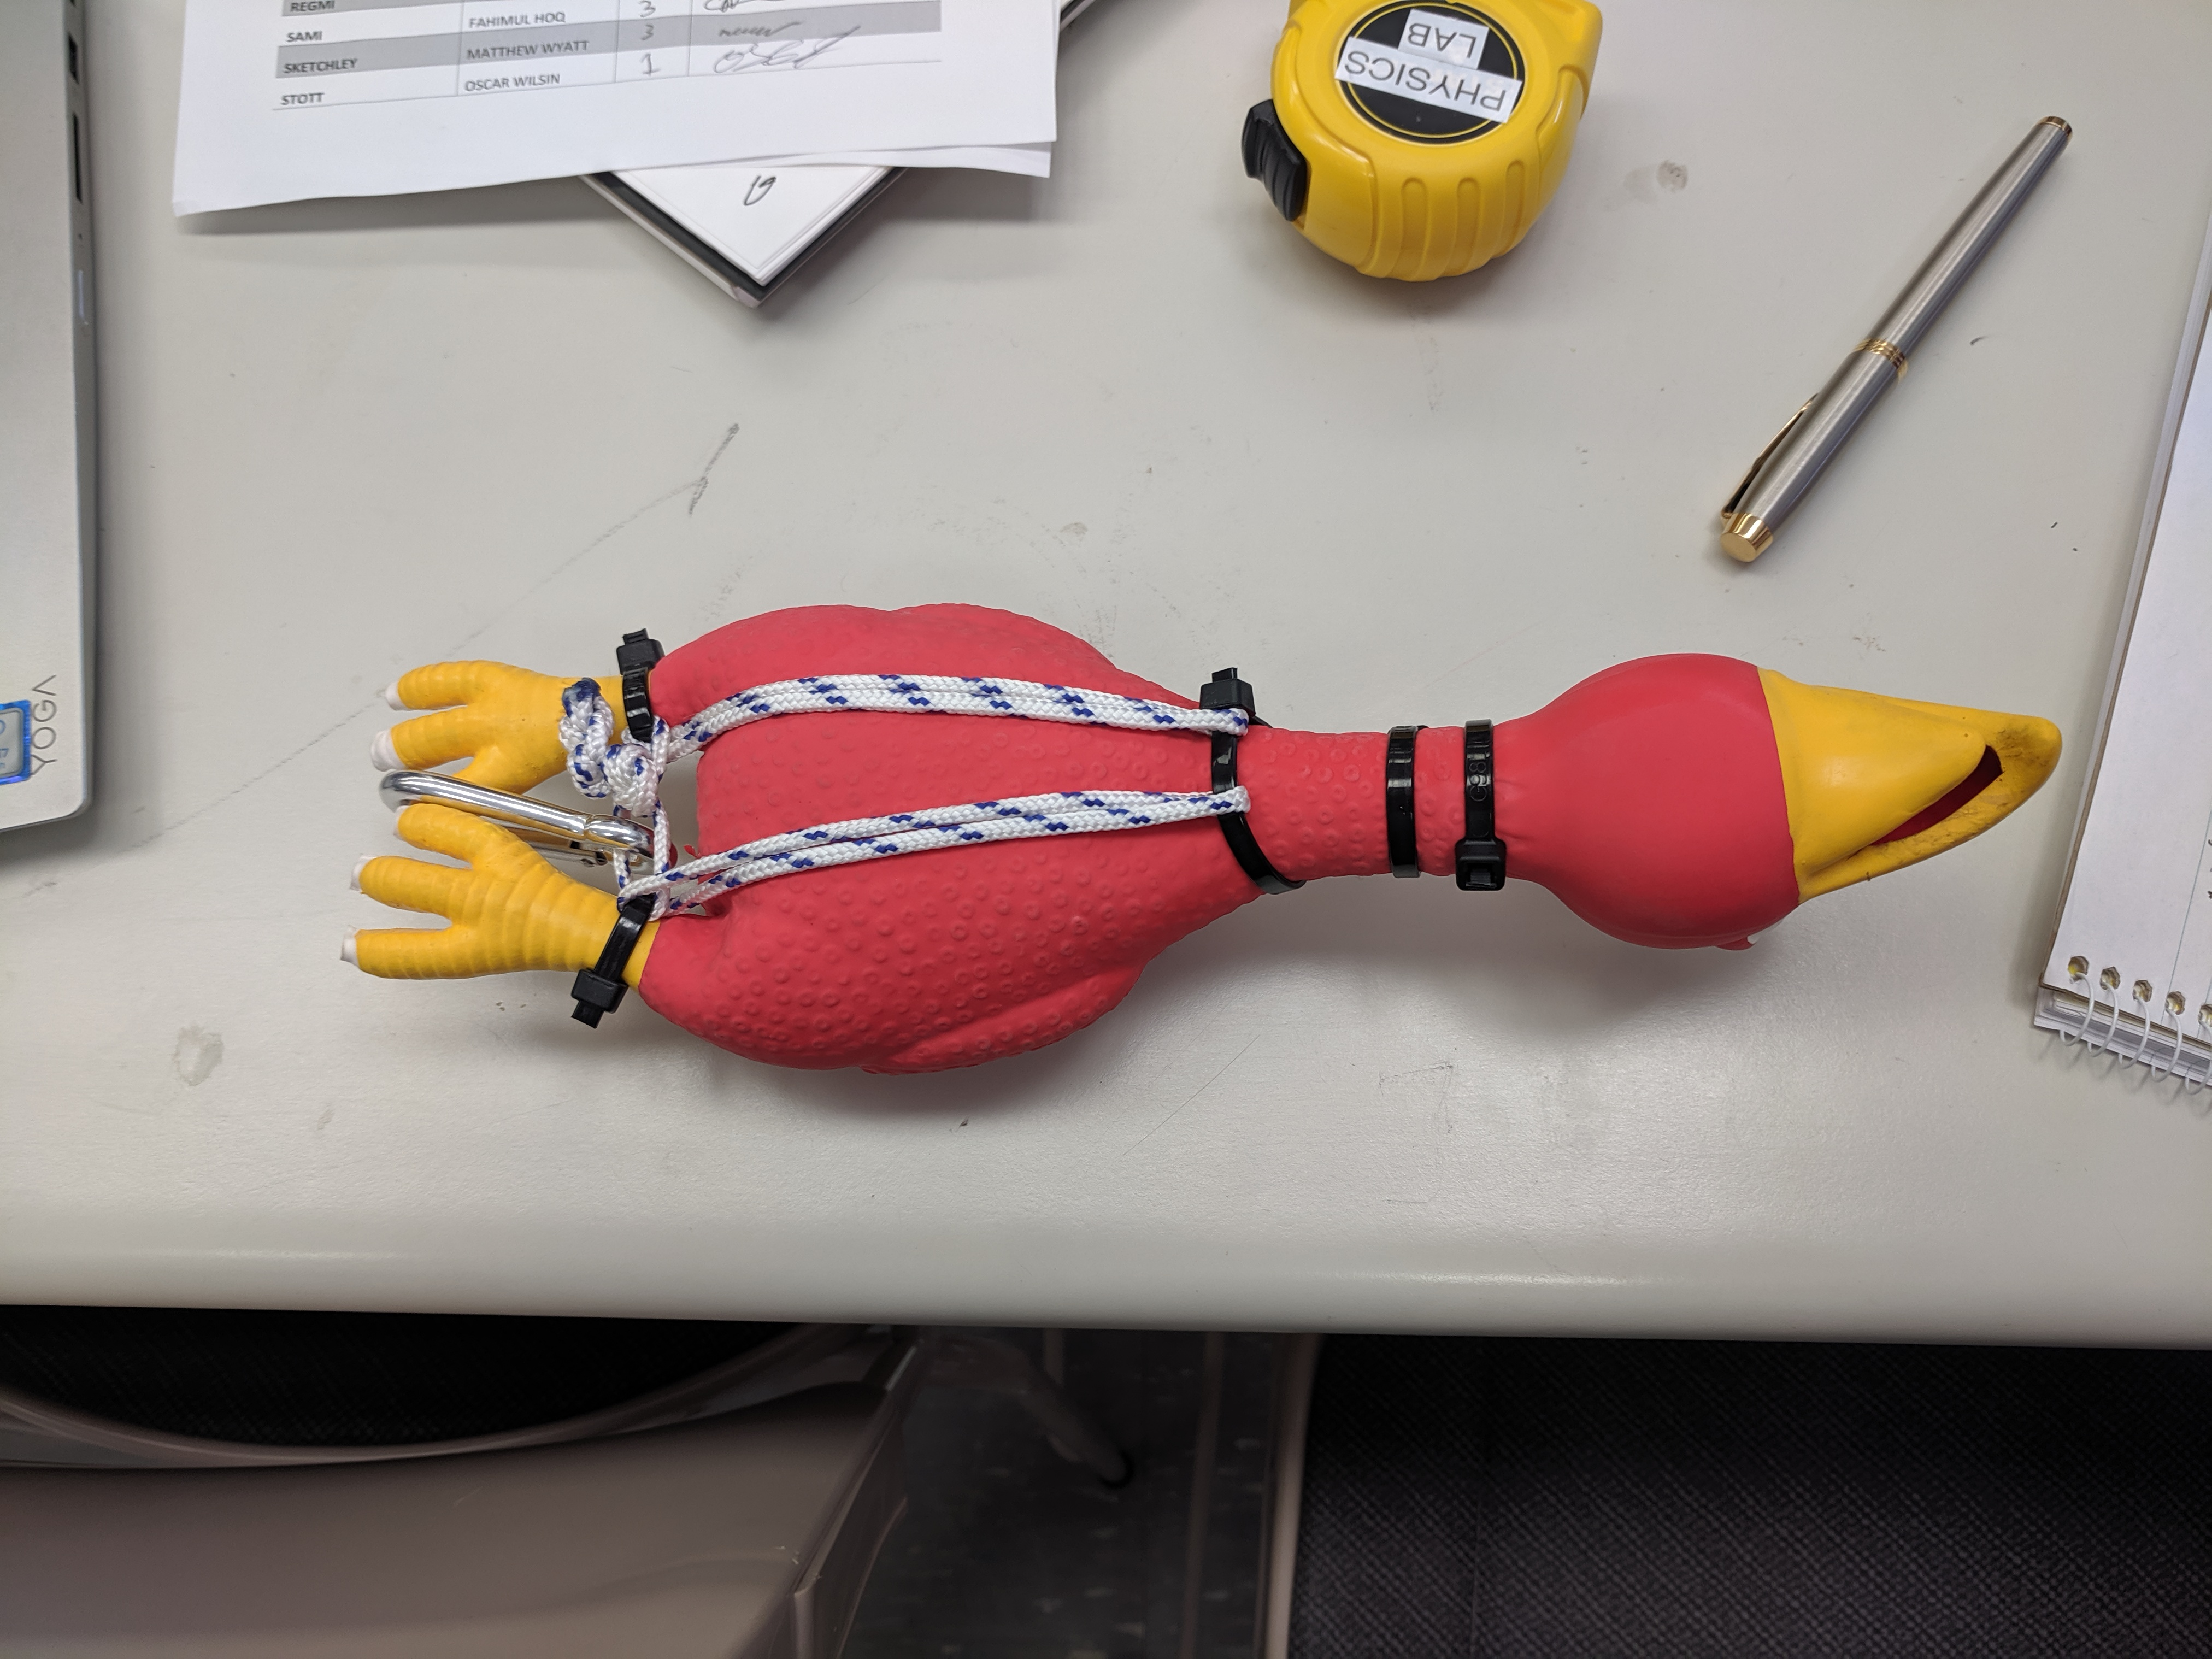
\includegraphics[scale=0.05]{chicken_1}}
		\caption{The rubber chicken that was used for the bungee jumping practical. The chicken mass was measured at 1.7kg, and the length from head to toe was measured at 0.33m}
	\end{minipage}
	\hspace{1cm}
	\begin{minipage}[t]{0.45\textwidth}
		\centering
		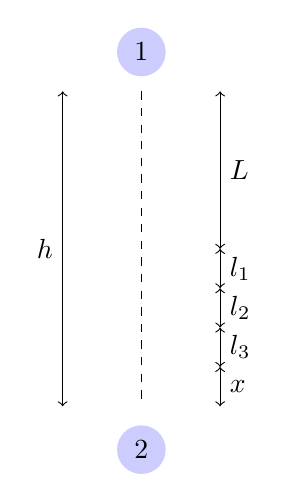
\begin{tikzpicture}
			\draw[dashed] (0,0) -- (0,-4);
			\node[circle,ultra thick, fill=blue!20] at (0,0.5) {1};
			\node[circle,ultra thick, fill=blue!20] at (0,-4.55) {2};
			\draw[<->] (-1,0) -- (-1,-4) node[midway, left] {$h$};
			\draw[<->] (1,0) -- (1,-2) node[midway, right] {$L$};
			\draw[<->] (1,-2) -- (1,-2.5) node[midway, right] {$l_1$};
			\draw[<->] (1,-2.5) -- (1,-3) node[midway, right] {$l_2$};
			\draw[<->] (1,-3) -- (1,-3.5) node[midway, right] {$l_3$};
			\draw[<->] (1,-3.5) -- (1,-4) node[midway, right] {$x$};
		\end{tikzpicture}
		\caption{In state 1, the chicken is at rest with no elastic potential energy. At state 2, the chicken is at rest, with no gravitational potential energy. All of the gravitational potential energy from state 1 has been transferred to elastic potential energy in state 2.}
	\end{minipage}
\end{figure}

Despite the complex dynamics occurring throughout the fall there are only two states of interest for calculating $L$: at rest immediately after being released; and at rest when the elastic cord has fully stretched and arrested the motion. These two states are denoted as state 1 and state 2, respectively and are graphically depicted in Figure XXXX. At state 1 we note that there is no elastic potential and the chicken is at rest. Similarly, at state 2 we note that there is no gravitational potential energy, and the chicken is again at rest, momentarily. We conclude that $(V_e)_1 = 0 \si{\joule}$; $T_1 = 0 \si{\joule}$; $(V_g)_2 = 0\si{\joule}$; and $T_2 = 0 \si{\joule}$, and the conservation of energy equation show in (XXXX) reduces to:
\begin{equation}
(V_g)_1 = (V_e)_2
\end{equation}

Using (XXXX) for gravitational potential energy, and (XXXX) for elastic potential energy we can re-express equation (12) as:
\begin{equation}
mgh = \frac{1}{2}kx^2
\end{equation}

Multiplying (XXXX) throughout by 2, and substituting (XXXX) results in the following:
\begin{equation}
2mgh = k\bigg(h - \sum_{i=1}^{3} l_i - L \bigg)^2
\end{equation}

Since $h$, $l_1$, $l_2$, and $l_3$ are all known we can simplify (14) by letting:
\begin{equation}
\eta = h - \sum_{i=1}^{3} l_i
\end{equation}

Hence, (XXXX) simplifies to:
\begin{equation}
\frac{2mgh}{k} = (\eta - L)^2
\end{equation}

The stiffness coefficient for an elastic cord of undetermined length can be expressed as $k = \sfrac{\xi}{L}$, where $\xi$ is experimentally determined. Hence, (XXXX) becomes:
\begin{equation}
\frac{2mgh}{\xi} L = (\eta - L)^2
\end{equation}

Expanding the right hand side of the equation and collecting like terms yields a quadratic expression in $L$:
\begin{equation}
L^2 - \bigg(2\eta + \frac{2mgh}{\xi}\bigg)L + \eta^2 = 0
\end{equation}

Finally, solving equation (XXXX) using the quadratic formula and simplifying yields:
\begin{equation}
L = \eta +\sfrac{mgh}{\xi} \pm \sqrt{(\eta + \sfrac{mgh}{\xi})^2 - \eta^2}
\end{equation}

Values for $h$, $l_1$, $l_2$, $l_3$, and $m$ were measured and can be found in Table XXXX below. The parameter $\xi$ was experimentally determined in Section XXXX and is listed in Table XXXX for reference, along with gravitational acceleration $g$. Calculated values for $L$, using (XXXX), can also be found in Table XXXX.
\begin{table}[h]
	\centering
	\caption{text}
	\begin{tabular}{lcrc}
		\toprule
		 Description & Parameter & Value & Unit\\
		\midrule
		 Height of balcony & $h$ & $8.81$ & $\si{\meter}$ \\
		 Length of chicken & $l_1$ & $0.05$ & $\si{\meter}$ \\
		 Length of tether & $l_2$ & $0.22$ & $\si{\meter}$ \\
		 Length of balcony connection & $l_3$ & $0.31$ & $\si{\meter}$ \\
		 Mass of chicken & $m$ & $1.70$ & $\si{\kilogram}$ \\
		 Experimentally derived stiffness & $\xi$ & $42.36$ & $\si{\newton}$ \\
		 Gravitational acceleration & $g$ & $9.81$ & $\si{\meter\per\second^2}$ \\
		 \midrule
		 \textbf{Calculated length of cord} & $L$ & $3.38$ & $\si{\meter}$\\
		 \bottomrule
	\end{tabular}
\end{table} 

\newpage

\section{Discussion}

\section{Conclusion}

\bibliography{my_bib}
\bibliographystyle{ieeetr}

\end{document}